\documentclass[11pt]{article}
\usepackage[margin=1in]{geometry}
\usepackage[T1]{fontenc}
\usepackage[utf8]{inputenc}
\usepackage{lmodern}
\usepackage{amsmath, amssymb}
\usepackage{graphicx}
\usepackage{hyperref}
\usepackage{float}
\usepackage{setspace}
\usepackage{caption}

\title{Quantifying Quantum Hallucinations in Language Models}
\author{Draft generated from the current experiment snapshot}
\date{\today}

\begin{document}
\maketitle
\onehalfspacing

\begin{abstract}
We evaluate whether language models produce physically inconsistent but superficially plausible answers on elementary quantum-mechanical tasks. We construct a controlled two-qubit benchmark with exact analytic ground truth for circuit evolution, operator composition, measurement prediction, and entanglement classification. Each model response is scored with a bounded normalized error metric $d_{phys} \in [0,1]$, where lower values are better. The current experiment covers 2{,}304 evaluations across three models, three prompted reasoning-depth settings, and four balanced task families. The resulting data show a clear size effect: larger models reduce mean physics error. In contrast, greater prompted reasoning depth yields only weak improvements, with uncertainty intervals that include zero. The largest errors occur on tasks requiring propagation of quantum states and probabilities through gate sequences. These results support a conservative conclusion: current language models can often generate structured quantum answers, but they remain unreliable when exact physical consistency is required.
\end{abstract}

\section{Introduction}
Large language models are increasingly used for scientific reasoning, coding, and mathematical problem solving. Quantum information tasks are a useful stress test for such systems because correctness is tightly constrained by linear algebra, normalization, unitarity, and the Born rule. A model may therefore produce an answer that appears well formed while still violating exact quantum-mechanical ground truth.

This paper studies that failure mode, which we refer to operationally as a \emph{quantum hallucination}: a syntactically plausible output that conflicts with exact quantum mechanics or with the target answer derived from exact simulation. Our goal is not to claim that language models fail universally on quantum tasks, but to measure how frequently they fail on a controlled family of simple tasks and to test whether those failures diminish with model scale or with prompted reasoning depth.

\section{Benchmark and Metric}
\subsection{Task families}
The benchmark uses four categories of exact two-qubit tasks:
\begin{itemize}
\item \textbf{Circuit evolution}: given an initial basis state and a sampled gate sequence, return the final state vector.
\item \textbf{Operator composition}: compose a one-qubit gate sequence and return the resulting unitary matrix.
\item \textbf{Measurement prediction}: compute the exact measurement probabilities after a gate sequence.
\item \textbf{Entanglement classification}: determine whether a given two-qubit state is entangled.
\end{itemize}

Ground truth is produced analytically inside the evaluation harness by explicit matrix multiplication over fixed gate sets. No external labels are used. This means the benchmark is self-labeled, reproducible, and exact within floating-point precision.

\subsection{Physics-grounded error}
For each response we compute a bounded error score $d_{phys}$:
\begin{itemize}
\item state-vector tasks compare the returned state to the exact target up to global phase and normalization penalties,
\item operator tasks combine deviation from the target operator with a unitarity penalty,
\item probability tasks compare the returned distribution to the exact Born-rule probabilities,
\item entanglement tasks use binary error.
\end{itemize}

By construction, $d_{phys}=0$ is correct and larger values indicate more severe physical inconsistency.

\subsection{Scaling law}
We model the expected error using
\[
\mathbb{E}[d_{phys}] = k S^{-\alpha} D^{\beta},
\]
where $S$ is a proxy for model size and $D$ is the prompted reasoning-depth condition. Parameters are estimated in log-linear form and accompanied by bootstrap confidence intervals.

\section{Experimental Setup}
The current snapshot evaluates three models: \texttt{gpt-4o-mini}, \texttt{gpt-4.1-mini}, and \texttt{gpt-4.1}. Each model is tested at prompted depth settings $D \in \{1,2,4\}$. The benchmark contains 64 prompts per category, yielding 256 unique prompts total and 2{,}304 scored evaluations after crossing prompts with models and depths.

The live results fragment used below is generated directly from the current JSON artifacts in the workspace. Updating the statistics file therefore updates this manuscript without manual copying.

\section{Results}
The main result is that physics-grounded error remains high across all tested models, but decreases with model size. The overall mean error is 0.497, and the best model in the current run still has mean error 0.442. This is not a rare-edge-case phenomenon: the 90th and 95th percentiles are both 1.0, and roughly one third of all samples are effectively full-error failures.

Among task families, circuit evolution and measurement prediction are the dominant sources of error. These are exactly the tasks that require maintaining correct quantum dynamics and probability propagation through gates. By contrast, entanglement classification and operator composition are easier on average, although even there the models remain imperfect.

The size trend is the strongest robust effect in the current experiment. The fitted exponent on model size is $\alpha \approx 1.993$ with a bootstrap 95\% confidence interval of $[1.509, 2.462]$. The direction is therefore stable across resamples. The depth effect is much weaker: $\beta \approx -0.290$ with a 95\% confidence interval of $[-0.876, 0.327]$, which includes zero. The safest interpretation is that larger models help, while additional prompted reasoning depth does not yet show a reliably strong benefit.

% Auto-generated by update_results_tex.py. Do not edit manually.
% Generated at 2026-04-03 09:56:49
\subsection*{Running Results Snapshot}
This fragment is generated directly from \texttt{paper\_quantum\_results.json} and \texttt{paper\_quantum\_fit.json}.

The current finished run contains 2304 usable evaluations. The overall mean normalized error is 0.497, with median 0.500, 90th percentile 1.000, and 95th percentile 1.000. Exact-correct outputs occur on 0.258 of samples, while 0.327 of samples are effectively full-error failures.
The best model by mean error is \texttt{gpt-4.1} (0.442), while the weakest is \texttt{gpt-4o-mini} (0.570). The best depth setting is 4 with mean error 0.483. The hardest category is \texttt{circuit\_evolution} (0.737), and the easiest is \texttt{entanglement\_classification} (0.304).
The fitted scaling law is $d_{phys} \approx k S^{-1.993} D^{-0.290}$, with $\alpha=1.993 [1.509, 2.462]$ and $\beta=-0.290 [-0.876, 0.327]$.

\subsubsection*{Overall Summary}
\begin{tabular}{lr}
\hline
Metric & Value \\
\hline
Usable evaluations & 2304 \\
Mean $d_{phys}$ & 0.497 \\
Median $d_{phys}$ & 0.500 \\
$p_{90}$ & 1.000 \\
$p_{95}$ & 1.000 \\
Exact-correct rate & 0.258 \\
$d_{phys} \ge 0.5$ rate & 0.506 \\
Full-error rate & 0.327 \\
\hline
\end{tabular}

\subsubsection*{By Model}
\begin{tabular}{lrrrrrr}
\hline
Model & $n$ & Mean & Median & 95\% CI & Zero rate & Full-error rate \\
\hline
gpt-4.1 & 768 & 0.442 & 0.354 & [0.412, 0.471] & 0.311 & 0.293 \\
gpt-4.1-mini & 768 & 0.478 & 0.461 & [0.449, 0.507] & 0.285 & 0.311 \\
gpt-4o-mini & 768 & 0.570 & 0.500 & [0.543, 0.598] & 0.177 & 0.378 \\
\hline
\end{tabular}

\subsubsection*{By Depth}
\begin{tabular}{rrrrrrr}
\hline
Depth & $n$ & Mean & Median & 95\% CI & Zero rate & Full-error rate \\
\hline
1 & 768 & 0.503 & 0.500 & [0.474, 0.532] & 0.250 & 0.336 \\
2 & 768 & 0.504 & 0.500 & [0.475, 0.533] & 0.251 & 0.329 \\
4 & 768 & 0.483 & 0.500 & [0.454, 0.512] & 0.272 & 0.316 \\
\hline
\end{tabular}

\subsubsection*{By Category}
\begin{tabular}{lrrrrrr}
\hline
Category & $n$ & Mean & Median & $p_{90}$ & Zero rate & Full-error rate \\
\hline
circuit\_evolution & 576 & 0.737 & 1.000 & 1.000 & 0.130 & 0.507 \\
entanglement\_classification & 576 & 0.304 & 0.000 & 1.000 & 0.696 & 0.304 \\
measurement\_prediction & 576 & 0.633 & 0.750 & 1.000 & 0.177 & 0.486 \\
operator\_composition & 576 & 0.313 & 0.354 & 0.500 & 0.028 & 0.012 \\
\hline
\end{tabular}

\subsubsection*{Pairwise Model Improvements}
\begin{tabular}{lrr}
\hline
Comparison & Absolute gain & Relative gain \\
\hline
gpt-4.1-mini & 0.093 & 0.162 \\
gpt-4.1 & 0.129 & 0.226 \\
gpt-4.1 vs gpt-4.1-mini & 0.036 & 0.076 \\
\hline
\end{tabular}

\subsubsection*{Best and Worst Model-Category Cells}
\begin{itemize}
\item Best: \texttt{gpt-4.1} on \texttt{entanglement\_classification} with mean 0.234 and 95\% CI [0.174, 0.294].
\item Best: \texttt{gpt-4.1-mini} on \texttt{entanglement\_classification} with mean 0.240 and 95\% CI [0.179, 0.300].
\item Best: \texttt{gpt-4.1} on \texttt{operator\_composition} with mean 0.283 and 95\% CI [0.260, 0.307].
\item Worst: \texttt{gpt-4o-mini} on \texttt{measurement\_prediction} with mean 0.711 and 95\% CI [0.666, 0.756].
\item Worst: \texttt{gpt-4.1-mini} on \texttt{circuit\_evolution} with mean 0.728 and 95\% CI [0.680, 0.776].
\item Worst: \texttt{gpt-4o-mini} on \texttt{circuit\_evolution} with mean 0.786 and 95\% CI [0.740, 0.831].
\end{itemize}

\subsubsection*{Model by Depth}
\begin{tabular}{lrrrrr}
\hline
Model & Depth & Mean & Median & Zero rate & Full-error rate \\
\hline
gpt-4.1 & 1 & 0.447 & 0.354 & 0.301 & 0.301 \\
gpt-4.1 & 2 & 0.441 & 0.354 & 0.316 & 0.281 \\
gpt-4.1 & 4 & 0.438 & 0.354 & 0.316 & 0.297 \\
gpt-4.1-mini & 1 & 0.480 & 0.471 & 0.285 & 0.320 \\
gpt-4.1-mini & 2 & 0.487 & 0.460 & 0.277 & 0.320 \\
gpt-4.1-mini & 4 & 0.466 & 0.423 & 0.293 & 0.293 \\
gpt-4o-mini & 1 & 0.582 & 0.500 & 0.164 & 0.387 \\
gpt-4o-mini & 2 & 0.583 & 0.500 & 0.160 & 0.387 \\
gpt-4o-mini & 4 & 0.546 & 0.500 & 0.207 & 0.359 \\
\hline
\end{tabular}

\subsubsection*{Model by Category}
\begin{tabular}{llrrrrr}
\hline
Model & Category & Mean & Median & 95\% CI & Zero rate & Full-error rate \\
\hline
gpt-4.1 & circuit\_evolution & 0.697 & 0.896 & [0.641, 0.753] & 0.182 & 0.500 \\
gpt-4.1 & entanglement\_classification & 0.234 & 0.000 & [0.174, 0.294] & 0.766 & 0.234 \\
gpt-4.1 & measurement\_prediction & 0.552 & 0.500 & [0.490, 0.614] & 0.260 & 0.438 \\
gpt-4.1 & operator\_composition & 0.283 & 0.344 & [0.260, 0.307] & 0.036 & 0.000 \\
gpt-4.1-mini & circuit\_evolution & 0.728 & 0.750 & [0.680, 0.776] & 0.099 & 0.464 \\
gpt-4.1-mini & entanglement\_classification & 0.240 & 0.000 & [0.179, 0.300] & 0.760 & 0.240 \\
gpt-4.1-mini & measurement\_prediction & 0.635 & 1.000 & [0.574, 0.696] & 0.250 & 0.542 \\
gpt-4.1-mini & operator\_composition & 0.308 & 0.354 & [0.285, 0.331] & 0.031 & 0.000 \\
gpt-4o-mini & circuit\_evolution & 0.786 & 1.000 & [0.740, 0.831] & 0.109 & 0.557 \\
gpt-4o-mini & entanglement\_classification & 0.438 & 0.000 & [0.367, 0.508] & 0.562 & 0.438 \\
gpt-4o-mini & measurement\_prediction & 0.711 & 0.750 & [0.666, 0.756] & 0.021 & 0.479 \\
gpt-4o-mini & operator\_composition & 0.347 & 0.354 & [0.321, 0.373] & 0.016 & 0.036 \\
\hline
\end{tabular}

\subsubsection*{Detailed Cell Rates (Model, Category, Depth)}
\begin{tabular}{llrrrrrr}
\hline
Model & Category & Depth & $n$ & Mean & Zero rate & $d_{phys} \ge 0.5$ & Full-error rate \\
\hline
gpt-4.1 & circuit\_evolution & 1 & 64 & 0.701 & 0.156 & 0.766 & 0.516 \\
gpt-4.1 & circuit\_evolution & 2 & 64 & 0.701 & 0.188 & 0.797 & 0.469 \\
gpt-4.1 & circuit\_evolution & 4 & 64 & 0.688 & 0.203 & 0.766 & 0.516 \\
gpt-4.1 & entanglement\_classification & 1 & 64 & 0.234 & 0.766 & 0.234 & 0.234 \\
gpt-4.1 & entanglement\_classification & 2 & 64 & 0.234 & 0.766 & 0.234 & 0.234 \\
gpt-4.1 & entanglement\_classification & 4 & 64 & 0.234 & 0.766 & 0.234 & 0.234 \\
gpt-4.1 & measurement\_prediction & 1 & 64 & 0.562 & 0.250 & 0.641 & 0.453 \\
gpt-4.1 & measurement\_prediction & 2 & 64 & 0.547 & 0.266 & 0.641 & 0.422 \\
gpt-4.1 & measurement\_prediction & 4 & 64 & 0.547 & 0.266 & 0.625 & 0.438 \\
gpt-4.1 & operator\_composition & 1 & 64 & 0.289 & 0.031 & 0.109 & 0.000 \\
gpt-4.1 & operator\_composition & 2 & 64 & 0.280 & 0.047 & 0.109 & 0.000 \\
gpt-4.1 & operator\_composition & 4 & 64 & 0.281 & 0.031 & 0.156 & 0.000 \\
gpt-4.1-mini & circuit\_evolution & 1 & 64 & 0.754 & 0.094 & 0.875 & 0.500 \\
gpt-4.1-mini & circuit\_evolution & 2 & 64 & 0.730 & 0.094 & 0.828 & 0.453 \\
gpt-4.1-mini & circuit\_evolution & 4 & 64 & 0.699 & 0.109 & 0.766 & 0.438 \\
gpt-4.1-mini & entanglement\_classification & 1 & 64 & 0.234 & 0.766 & 0.234 & 0.234 \\
gpt-4.1-mini & entanglement\_classification & 2 & 64 & 0.250 & 0.750 & 0.250 & 0.250 \\
gpt-4.1-mini & entanglement\_classification & 4 & 64 & 0.234 & 0.766 & 0.234 & 0.234 \\
gpt-4.1-mini & measurement\_prediction & 1 & 64 & 0.633 & 0.250 & 0.703 & 0.547 \\
gpt-4.1-mini & measurement\_prediction & 2 & 64 & 0.664 & 0.234 & 0.719 & 0.578 \\
gpt-4.1-mini & measurement\_prediction & 4 & 64 & 0.609 & 0.266 & 0.703 & 0.500 \\
gpt-4.1-mini & operator\_composition & 1 & 64 & 0.298 & 0.031 & 0.125 & 0.000 \\
gpt-4.1-mini & operator\_composition & 2 & 64 & 0.304 & 0.031 & 0.094 & 0.000 \\
gpt-4.1-mini & operator\_composition & 4 & 64 & 0.323 & 0.031 & 0.141 & 0.000 \\
gpt-4o-mini & circuit\_evolution & 1 & 64 & 0.790 & 0.094 & 0.906 & 0.547 \\
gpt-4o-mini & circuit\_evolution & 2 & 64 & 0.794 & 0.094 & 0.891 & 0.547 \\
gpt-4o-mini & circuit\_evolution & 4 & 64 & 0.772 & 0.141 & 0.844 & 0.578 \\
gpt-4o-mini & entanglement\_classification & 1 & 64 & 0.484 & 0.516 & 0.484 & 0.484 \\
gpt-4o-mini & entanglement\_classification & 2 & 64 & 0.484 & 0.516 & 0.484 & 0.484 \\
gpt-4o-mini & entanglement\_classification & 4 & 64 & 0.344 & 0.656 & 0.344 & 0.344 \\
gpt-4o-mini & measurement\_prediction & 1 & 64 & 0.711 & 0.031 & 0.891 & 0.484 \\
gpt-4o-mini & measurement\_prediction & 2 & 64 & 0.703 & 0.016 & 0.875 & 0.469 \\
gpt-4o-mini & measurement\_prediction & 4 & 64 & 0.719 & 0.016 & 0.906 & 0.484 \\
gpt-4o-mini & operator\_composition & 1 & 64 & 0.343 & 0.016 & 0.203 & 0.031 \\
gpt-4o-mini & operator\_composition & 2 & 64 & 0.351 & 0.016 & 0.203 & 0.047 \\
gpt-4o-mini & operator\_composition & 4 & 64 & 0.348 & 0.016 & 0.188 & 0.031 \\
\hline
\end{tabular}


\begin{figure}[H]
\centering
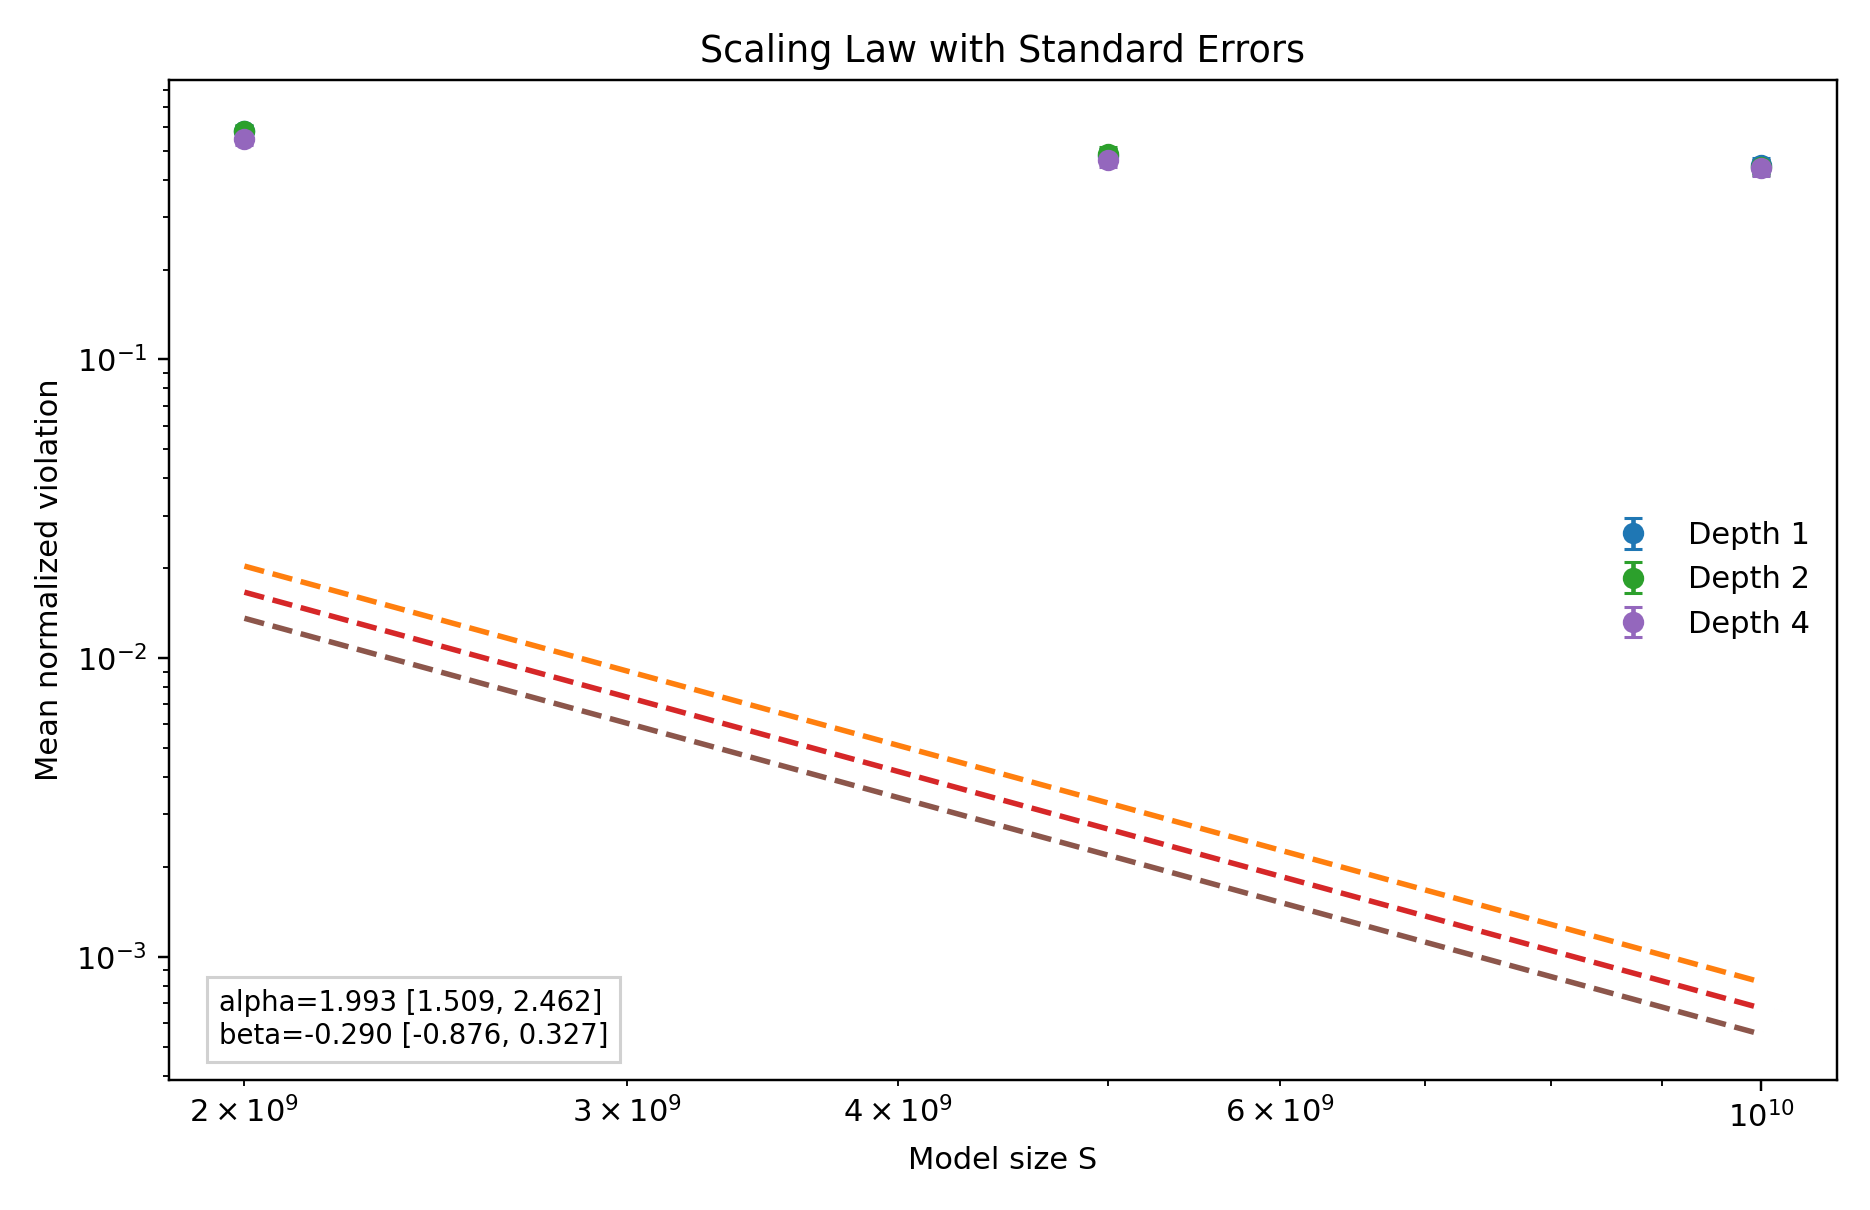
\includegraphics[width=0.82\textwidth]{paper_quantum_scaling.png}
\caption{Scaling-law figure generated from the current completed run. Error bars reflect within-cell variability, and the fitted trend is reported in the text.}
\label{fig:scaling}
\end{figure}

\begin{figure}[H]
\centering
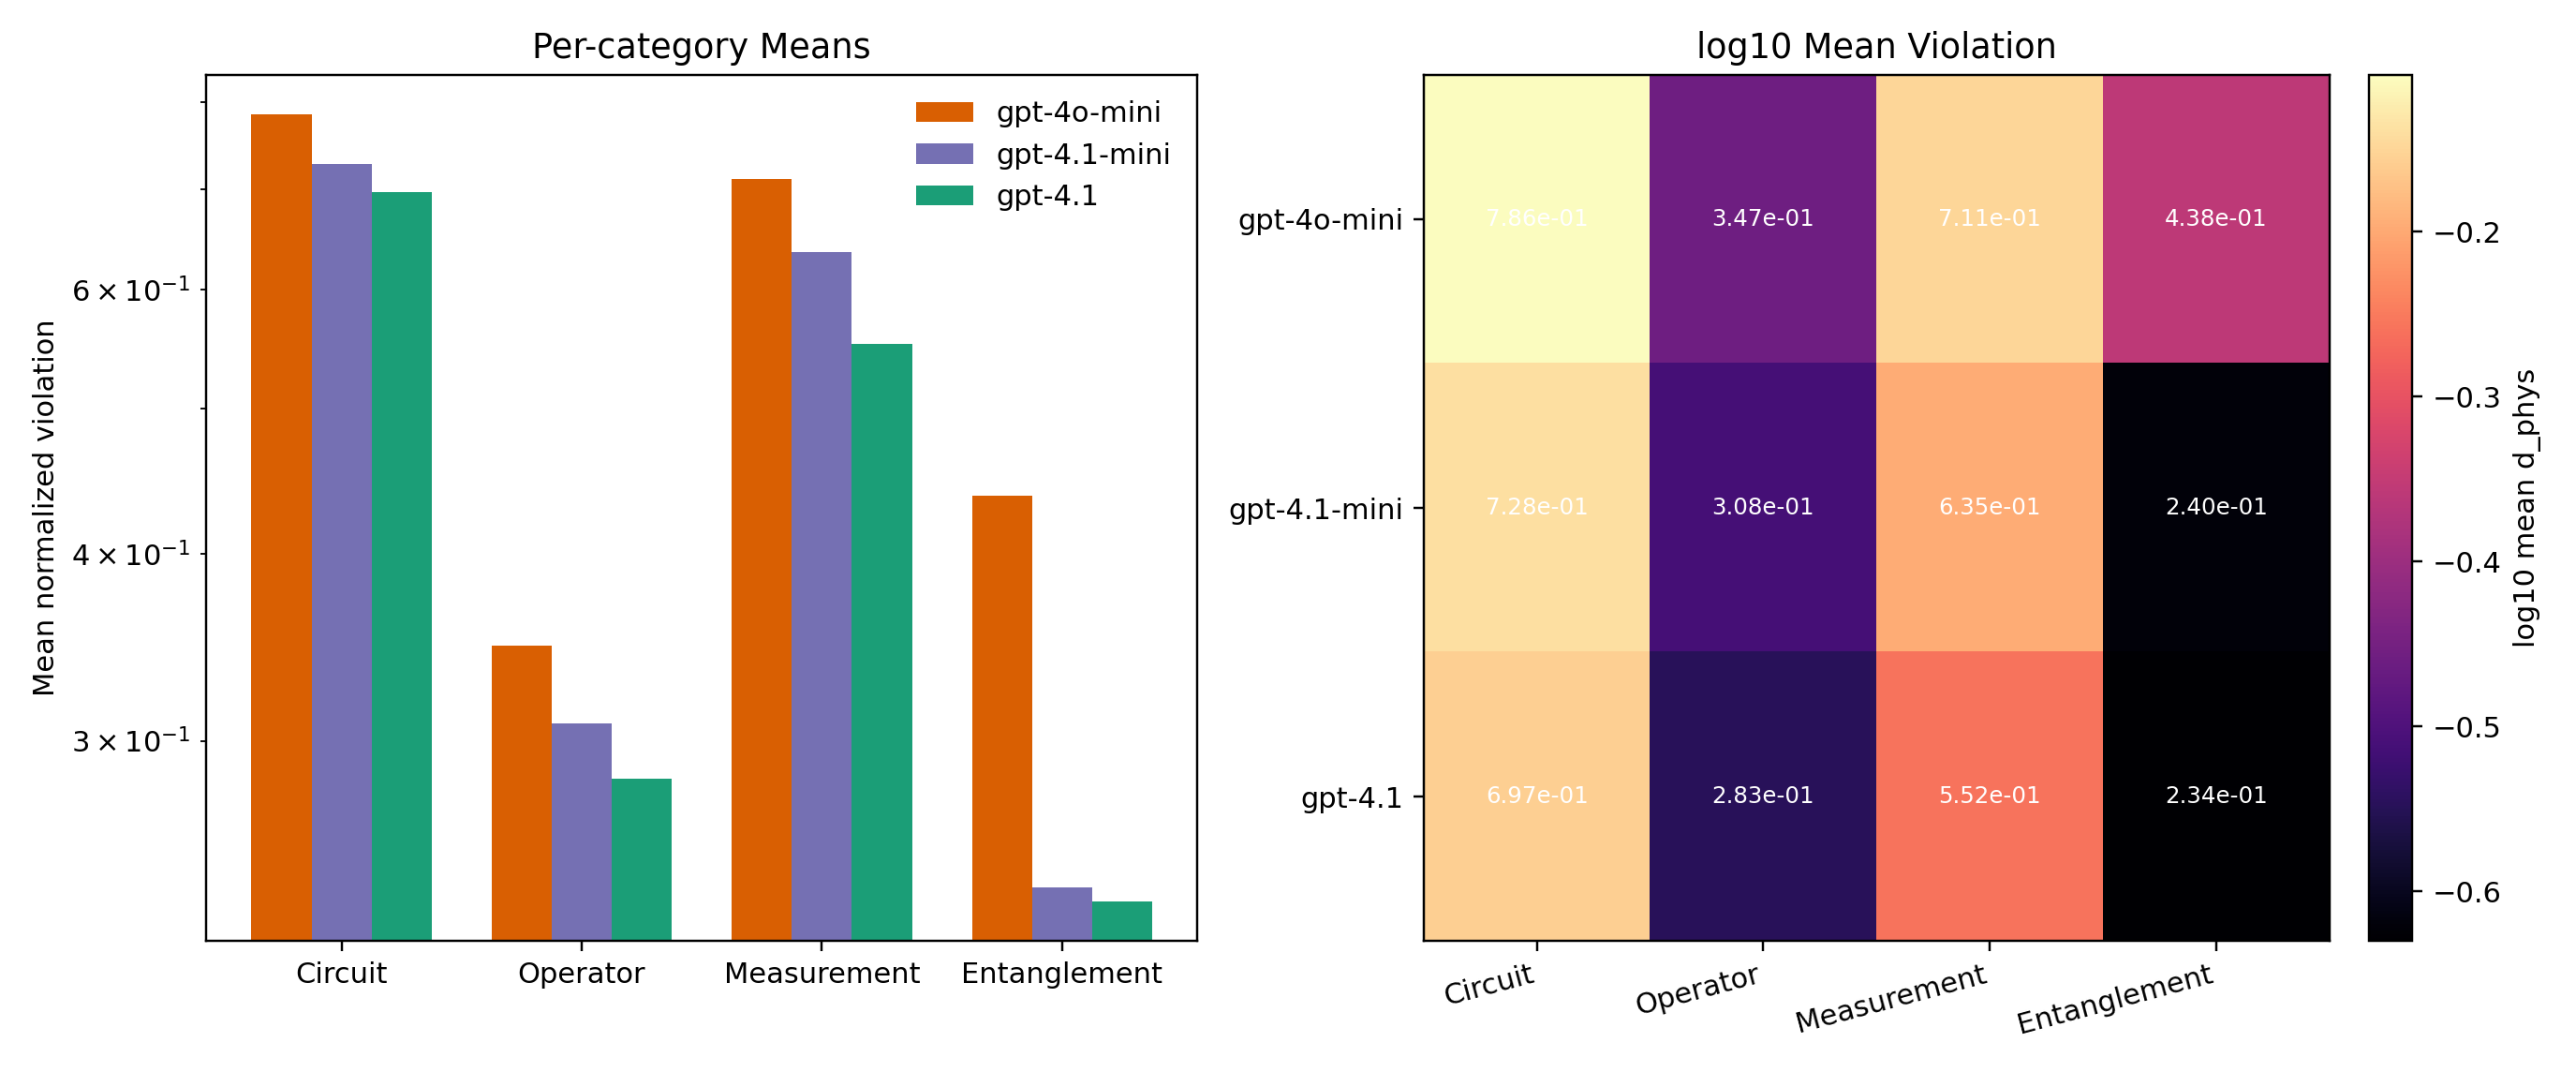
\includegraphics[width=\textwidth]{paper_quantum_breakdown.png}
\caption{Breakdown of mean normalized error by task family and model. The pattern highlights that circuit evolution and measurement prediction dominate the observed failure modes.}
\label{fig:breakdown}
\end{figure}

\section{Discussion}
The current snapshot supports three conservative claims.

First, language models can produce structured quantum answers while still being physically wrong. This is the operational sense in which the term \emph{hallucination} is used in this work: the output has the right surface form, but not the right physics.

Second, scale matters. The progression from \texttt{gpt-4o-mini} to \texttt{gpt-4.1-mini} to \texttt{gpt-4.1} lowers mean error, lowers full-error rate, and increases exact-correct rate. This indicates that the benchmark is sensitive to capability differences rather than merely to prompt formatting.

Third, prompting for more reasoning is not a substitute for stronger models. Depth 4 is marginally better on average than depths 1 and 2, but the effect is small relative to model-to-model differences and is not statistically stable in the current bootstrap interval.

\section{Limitations}
This draft is based on a controlled two-qubit benchmark. That makes exact scoring possible, but it also limits ecological scope. The size variable is a proxy rather than a verified parameter count, and the study uses a narrow family of model releases. In addition, the current manuscript reports a single benchmark configuration and does not yet include ablations over prompt phrasing, temperature, or alternative quantum task distributions.

\section{Conclusion}
The present experiment shows that current language models frequently fail elementary quantum tasks in ways that are physically meaningful, not merely stylistic. Larger models reduce these failures, but the remaining error is still substantial, especially for circuit evolution and measurement prediction. The current evidence therefore supports a measurement-oriented conclusion: language models can often produce plausible quantum answers, yet exact physical reliability remains limited.

\end{document}
